\subsection{What is the value of a model based on average feature values?}
\label{sec:mean-model}
I am not the first to observe that fitting a model to the mean of feature values across a distribution of cells of the same type may not result in a model that well-described an actual neuron from that distribution.
Neuron modelers have some awareness of this problem which has been thoroughly characterized in \cite{marder2011multiple}, though it remains underappreciated.
This is especially obvious when the feature distribution is multi-modal (such as inset-e in the figure below), but it could also result from hidden covariance structure among the features (Figure \ref{fig:eve_marder}).

\begin{figure}
\begin{center}

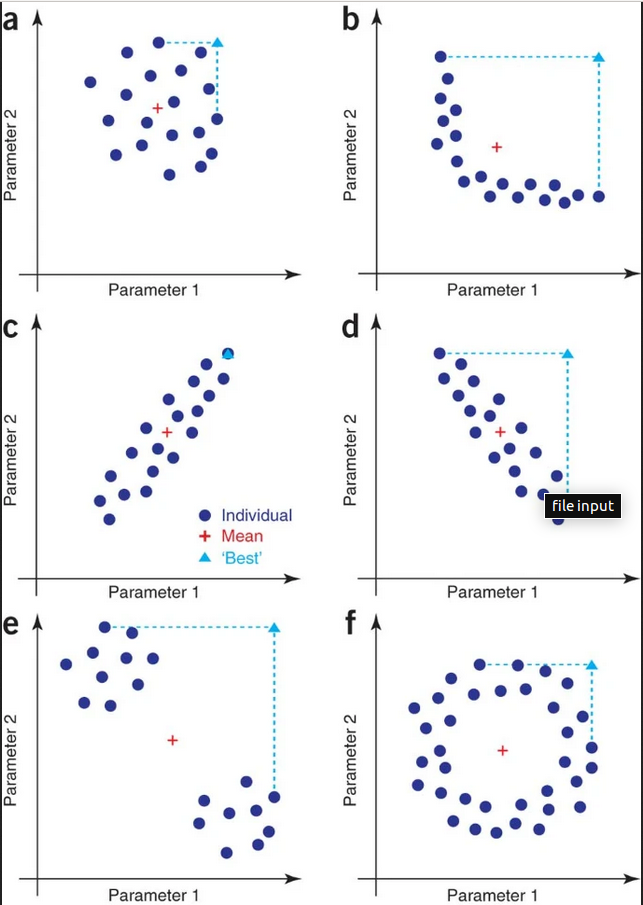
\includegraphics[scale=0.65]{figures/eve_marder.png}
\end{center}
\caption[Lessons from Marder]{ADD THIS CAPTION}
\label{fig:eve_marder}
\end{figure}


Previously in methods \ref{section:nelectro}, we showed that some feature distributions are bimodal.
Consider a cell type which had an underlying bimodal distribution for input resistance, with a mean exactly between the two modes.
If we optimize a neuron against this mean value, then the optimized neuron does not describe the modes (where most of the cells are actually located) at all.
Conversely, suppose that we optimize each neuron from the distribution individually, and then produce a model which just averages across the parameter values of each of these optimized models.
Its entirely conceivable that that this ``mean model" would produce measurements that were similar to the mean of the feature distribution.
However, when we are dealing with a nonlinear dynamical system, this is by no means certain (and perhaps not even likely).
This mean model could also exhibit much higher or lower feature values.
For example, we expect that even these comparatively simple reduced models have multiple regimes characterized by sharp transitions in parameter space between, for example, regular spiking behavior and bursting behavior, or tonic-bursting vs chattering.
What would it even mean to split the difference between two such fundamentally different regimes?

In order to examine this question further in the context of my optimizer applied to reduced models, I created two models from each model class (e.g. Izhikevich) with different sets of parameter values.
I simulated each of these models, computed all of the measurements associated with the core NeuronUnit tests (rheobase, input resistance, capacitance, and membrane time constant), and then simply averaged them together across the two models.
I call these the ``mean features" as each one reflects the mean across two parameterizations of the model.
In parallel, I also create a ``mean model" which reflects the average of the parameters themselves, and then measure the same set of features for this mean model.
I then ask the question: "Do the features from the mean model match the mean features?"
If these match nearly all of the time, we can feel confident that optimizing a model based on the mean features will produce a model that is representative of the parameter space of the neurons individually.
In other words, if we had access to the measurements from the individual neurons, and fit models to those, then the mean model obtained above should lie somewhere between those models in parameter space.
By contrast, if the mean model does not match the mean features, that would suggest that models obtained by optimizing against mean features may not be representative in this context.

The results are shown below.
In Figure \ref{fig:mean-model-1}, I show a representative example using two random locations in parameter space.
While some of the differences between the two parameter sets may look small, this is only a reflection of the scale being dominated by the parameters that intrinsically have the largest values.

\begin{figure}
\begin{center}
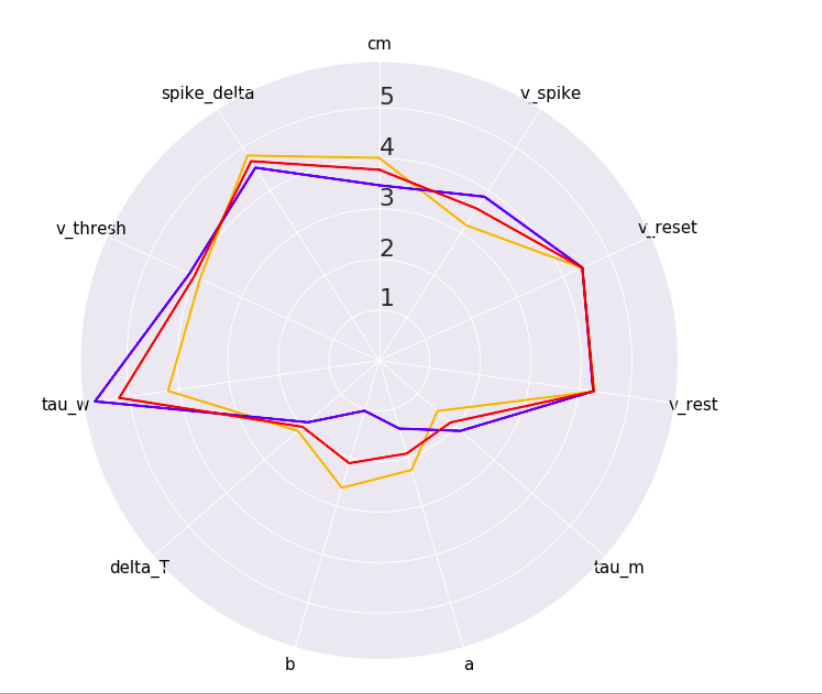
\includegraphics[]{figures/polar_coordinates.png}


\caption[Random model pair, and mean model]{Virtual Experiment setup. Red trace 'mean' coordinate model, blue trace model 'a', yellow trace model 'b'. Two random models are drawn from uniformly distributed random number generators in the AdEx model parameter range. The mean is taken from the pair of model coordinates, to get the mean set of coordinates. The polar coordinate plot shows this mean model as in between model a and model b. Note in the polar plots generally, each parameter and model measurement occupies disparate ranges of magnitude. Log and absolute value are used to in order to make the relevant proportions accessible, in this plot, but also in all preceding polar plots.}
\end{center}
\end{figure}


\begin{table}


\begin{adjustbox}{width=\columnwidth,center}

\begin{tabular}{lrrrrrrrrrrr}
\toprule {} &          cm &    v\_spike &    v\_reset &     v\_rest &      tau\_m &         a &          b &   delta\_T &       tau\_w &   v\_thresh &  spike\_delta \\
\midrule
a           &  954.283985 & -39.652421 & -33.290058 & -71.274552 &  18.409430 &  8.732663 &  13.449849 &  9.178972 &  205.178522 & -29.526272 &    69.811681 \\
b           &  885.614383 & -57.290057 & -57.805723 & -96.183985 &  51.917341 &  0.086329 &  13.464095 &  8.315697 &  271.050894 & -58.339164 &    93.170984 \\
mean of a and b &  919.949184 & -48.471239 & -45.547891 & -83.729269 &  35.163385 &  4.409496 &  13.456972 &  8.747335 &  238.114708 & -43.932718 &    81.491333 \\
\bottomrule
\end{tabular}
\end{adjustbox}
\caption[coordinate information in tabular form]{The same polar coordinates in tabular form.}
\end{table}



\begin{figure}
    \centering
    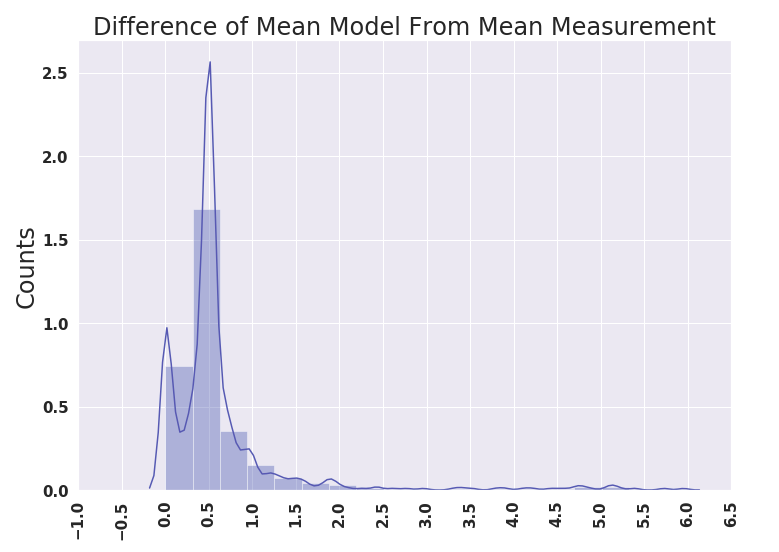
\includegraphics{figures/mean_model_vs_mean_measurement.png}
    \caption[100 pairs of randomly sampled AdEx models: mean model mean parameter difference]{100 pairs of randomly sampled AdEx models: mean model mean parameter difference. The value 0.5 signifies midway distance between model 'a' and model 'b'. The majority of histogram counts fall at $~0.5$, but also a significant number of mean models do not agree with the mean of a and b..}
    \label{fig:mean-model-1}
\end{figure}


\begin{figure}
    \centering
    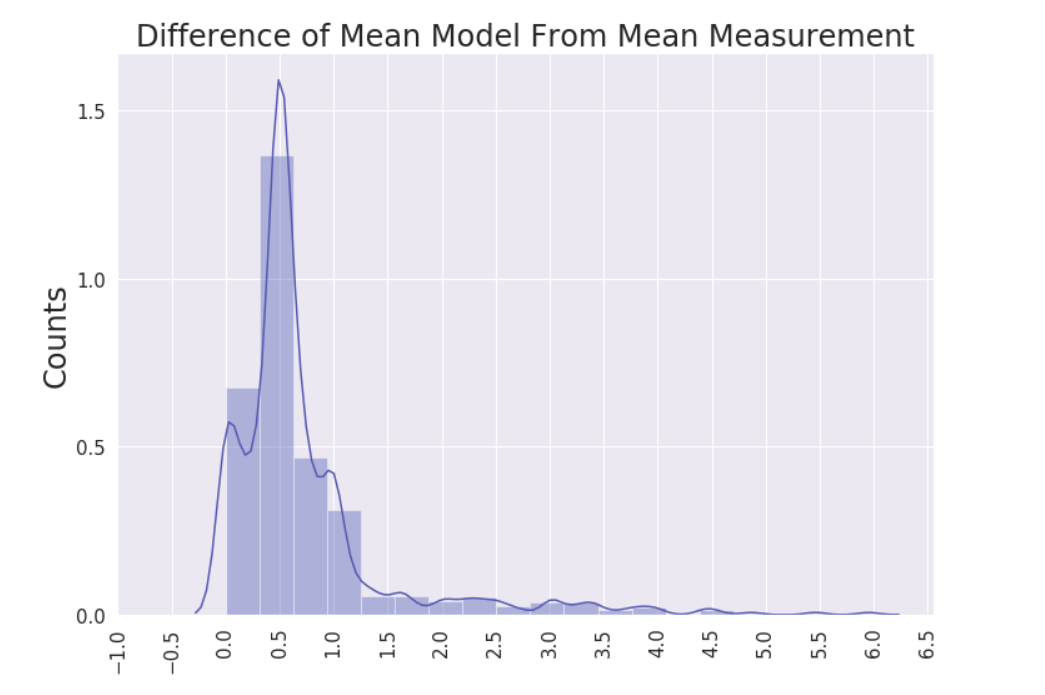
\includegraphics{figures/reproduced_izhi.png}
    \caption[100 pairs of randomly sampled Izhikevich models: mean model mean parameter difference]{This plot essentially reproduces the findings of the above analysis, but in a different model type. This time the Izhikevich model was used. The Izhikevich model demonstrates more values that are above or below $0.5$, this is expected, because the implementation of the Izhikevich model is not static, to better model various regimes, the Izhikevich model draws upon slightly different versions of governing equations. Therefore slightly different versions of the model governing equations were randomly sampled. The average of two models, that exist between explicitly different equations, are much less likely to result in average measurements at $0.5$}
    \label{fig:mean-model-2}
\end{figure}

Although the peak identified in fig(\label{fig:mean-model-2}), looks taller in absolute size compared to (fig {fig:mean-model-1}), the scale along the y-axis is different. Actually {fig:mean-model-1} has more histogram counts at 0.5.




\begin{figure}
    \centering
    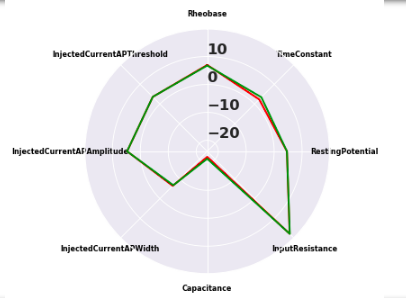
\includegraphics{figures/model_similarities.png}
        \label{fig:mean-model-1}
    \caption[Here I plot some single instance of mean model mean measurement discrepancy]{Since a larger proportion of models agree (produce mean models that are positioned midway between model a and model b, here I show an example of mean model and mean measurement agreement. The distribution plot above is made up of 100 different instances of random model pairs and mean models. There are some small discrepancies visible, but generally most measurements are closely matched}
\end{figure}

\begin{figure}
    \centering
    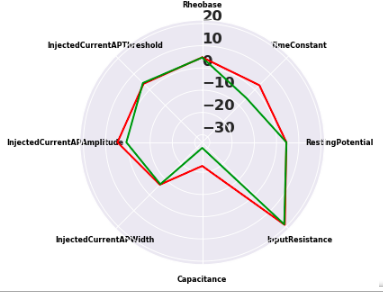
\includegraphics{figures/model_differences.png}
        \label{fig:mean-model-1}
    \caption[Disparity in mean model, mean measurement agreement]{This time I show a common pattern of disagreement, between mean model and mean measurement. The most prominent discrepencies of measurement are in Capacitance, TimeConstant, and InjectCurrentAPAmplitude}
\end{figure}

\begin{figure}
    \centering
    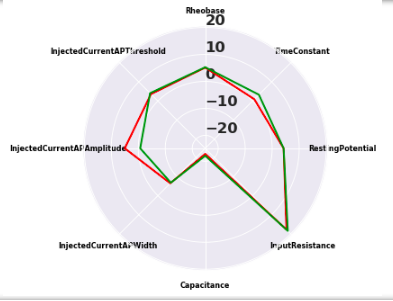
\includegraphics{figures/model_differences2.png}
        \label{fig:mean-model-1}
    \caption[Second example of disparity in mean model, mean measurement agreement]{This time I show a less common pattern of disagreement, between mean model and mean measurement.}
\end{figure}


%\begin{figure}
%    \centering
%    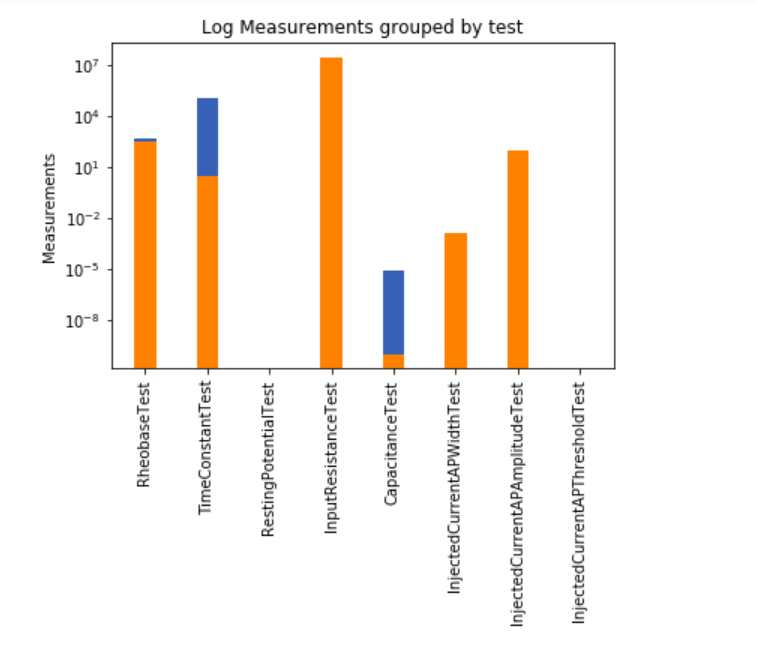
\includegraphics{figures/mean_model_mean_test.png}
%    \caption{Caption}
%    \label{fig:my_label}
%\end{figure}

In Figure \ref{fig:mean-model-2}, I show the computed feature values from simulations of each of the three models in Fig. \ref{fig:mean-model-1}.
While in some cases the mean model produces feature values that lie between (are equal to the mean of) the feature values of the original two models, in other cases there is a massive discrepancy.

In conclusion, it is not safe to assume that the parameters space and the feature space are isomorphic, and thus fitting models to the mean feature values for a distribution of neurons is a dangerous exercise even if the data themselves are normal-like.

%\begin{figure}
%    \centering
%    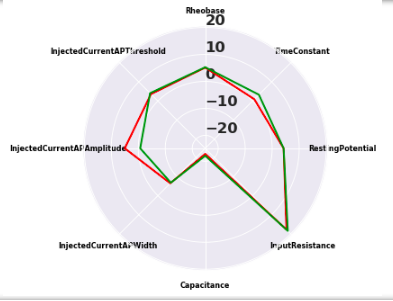
\includegraphics{figures/model_differences2.png}
%        \label{fig:mean-model-1}
%    \caption[Second example of disparity in mean model, mean measurement agreement]{This time I show a less common pattern of disagreement, between mean model and mean measurement.}
%\end{figure}

%\begin{comment}
%\begin{figure}
%    \centering
%    \includegraphics{figures/mean%_model_mean_test2.png}
%    \caption[bar charts that reveal disparity between mean model and mean measurement]{A stacked bar chart was used and each bar was positioned to represent each of the different measurement types. Very often the mean model measurement, green, is at a comparable height as model a, b and the mean model. There are two glaring exceptions which are the time constant measurement, and the capacitance measurement. At those measurement locations the mean is significantly greater than the mean of model a and model b}
%    \label{fig:mean-model-2}
%\end{figure}
%\end{comment}

%explore if this was a problem for models as well as experimental cells.